\documentclass[journal]{IEEE/IEEEtran}
\usepackage{pkg/pgf-pie}
\usepackage[T1]{fontenc}
\usepackage{inconsolata}
\usepackage{graphicx}

\graphicspath{ {images/} }

\usepackage{color}

\definecolor{pblue}{rgb}{0.13,0.13,1}
\definecolor{pgreen}{rgb}{0,0.5,0}
\definecolor{pred}{rgb}{0.9,0,0}
\definecolor{pgrey}{rgb}{0.46,0.45,0.48}
\usepackage{cite,graphicx,pgfplots,amsmath}
\usepackage{listings}
\usepackage{blindtext}
\lstset{language=Java,
  showspaces=false,
  showtabs=false,
  breaklines=true,
  showstringspaces=false,
  breakatwhitespace=true,
  commentstyle=\color{pgreen},
  keywordstyle=\color{pblue},
  stringstyle=\color{pred},
  basicstyle=\ttfamily,
%  moredelim=[il][\textcolor{pgrey}]{$$},
  moredelim=[is][\textcolor{pgrey}]{\%\%}{\%\%}
}



\newcommand{\SPTITLE}{UPLB Network Queue Simulator (UNQS): Surveying Network Performance For Internet Bandwidth Management}
\newcommand{\ADVISEE}{Leensey M. Lawas}
\newcommand{\ADVISER}{Danilo J. Mercado}

\newcommand{\BSCS}{Bachelor of Science in Computer Science}
\newcommand{\ICS}{Institute of Computer Science}
\newcommand{\UPLB}{University of the Philippines Los Ba\~{n}os}
\newcommand{\REMARK}{\thanks{Presented to the Faculty of the \ICS, \UPLB\
                             in partial fulfillment of the requirements
                             for the Degree of \BSCS}}
        
\markboth{CMSC 200 Undergraduate Thesis, \ICS}{}
\title{\SPTITLE}
\author{\ADVISEE~and~\ADVISER%
\REMARK
}
\pubid{\copyright~2016~ICS \UPLB}

%%%%%%%%%%%%%%%%%%%%%%%%%%%%%%%%%%%%%%%%%%%%%%%%%%%%%%%%%%%%%%%%%%%%%%%%%%

\begin{document}

% TITLE
\maketitle

% ABSTRACT
\begin{abstract}
Given the increasing demand for bandwidth, UNQS was developed to survey and to identify the optimal bandwidth setting as measured by duration (seconds), throughput (bits per second), and flow loss (percentage). The results show that while the simplest, FIFO showed the  best performance with minimal duration, maximal throughput, and minimal packet loss.
\end{abstract}

% INDEX TERMS
\begin{keywords}
bandwidth management, internet, network performance, network simulation, queueing, traffic engineering
\end{keywords}

% INTRODUCTION
\section{Introduction}
With the prevalence of internet usage in this digital age, the rise of demand for fast and reliable execution of online services is inevitable. Whether it is for personal use, like video chatting with friends and family from abroad, or for commercial and business transactions, customers want to make sure their services are done efficiently without slowing down or timing out. Client requests are sent simultaneously that when the server responses (or traffic) are returned, the routers are unable to inspect long fields in Internet Protocol (IP) packet headers quickly and are unable to reassemble and segment packets fast enough, causing performance bottleneck \cite{pazos_gerla_rigolio_1999}. A quick solution to the problem would be increasing bandwidth size, because as the demand for services increases, the bandwidth must also be increased \cite{communication_news_2001}. However, this method is costly and inefficient, which is why traffic engineering (TE) takes place. 

Awduche, Chiu, Elwalid, Widjaja, and Xiao of The Internet Society (2002) \cite{awduche_chiu_elwalid_xiao_2002} defined that internet traffic engineering deals with evaluating network performance and optimizing it. Bandwidth is the unit of measurement, usually in Kbps or Mbps, used to monitor network performance for quantifying how much information a communication channel can handle \cite{teach_ict_nd}.

\subsection{Background of the study}
Tong and Yang (2007)\cite{tong_yang_2007} cited that there have been many studies on TE, but most of them dealt with route selection algorithms, and few tackled bandwidth management techniques. For this study, bandwidth management is the TE method chosen. Kanu, Kuyoro, Ogunlere, \& Adegbenjo \cite{kanu_kuyoro_ogunlere_adegbenjo_2012} define bandwidth management as an optimization technique that helps differentiate the types of network traffic from each other and determine which client or service should be prioritized. In short, bandwidth management allocates the available bandwidth depending on network traffic and client/service priority.

In an article named \textit{Bandwidth management pays off} (2002)\cite{communication_news_2001}, two key devices were identified to help in bandwidth management: traffic shaping or congestion avoidance mechanisms and queueing techniques. \textit{Congestion avoidance mechanisms} or \textit{congestion control} locates where in the router the packets do not enter the system, and finds an alternative route so the packets do not block the way and cause timeout \cite{jacobson_1988}. \textit{Queueing techniques}, on the other hand, help predict and direct the traffic flow by implementing a constraint or constraints to provide the services as demanded \cite{gross_harris_1974}). In addition, queueing network models are known for accuracy and efficiency \cite{lazowska_zahorjan_graham_sevcik_1984}.

\subsection{Significance of the study}
Inefficient internet bandwidth management can lead to dissatisfied customers and reduced productivity. As long there is a need for “high quality of corporate customer satisfaction”, bandwidth management will continue to grow as a body of knowledge \cite{duzbeck_2006}. This study simulated actual traffic data within the University of the Philippines Los Banos (UPLB) Network in order to determine whether the existing bandwidth is optimal or not. Additionally, the results can also be used for future planning that can entail significant cost reductions, thus optimizing both bandwidth and budget to provide quality service.

\subsection{Objectives of the study}
The general objective of the study is to efficiently simulate the UPLB network traffic by identifying the most optimal bandwidth setting. Specifically, the study was able to:

\begin{enumerate}
\item Collect traffic data from the UPLB network;
\item Simulate the traffic data using various bandwidth sizes;
\item Take note of the duration, throughput, and flow loss for each simulation; and
\item Determine the most optimal network setting using graphs and simple statistics.
\end{enumerate}

\clearpage

\subsection{Time and Place of the study}
The study was conducted from January 2017 until November 2017, at the Institute of Computer Science, UPLB.

\subsection{Scope and Limitation of the study}
The study is limited to monitoring and simulating a portion of the UPLB network. Also, it focused on the traditional queueing technique known as First In-First Out Queueing (FIFO).

In determining the most optimal bandwidth, the throughput, latency, and flow loss values will be measured, noted, and compared. \textit{Throughput} is the number of tasks accomplished over a period of time, \textit{latency} is the time it takes for a fixed task to be finished \cite{martin_roth_nd}, and \textit{flow loss} is the percentage of dropped flows over the total number of flows.

\section{Review of Related Literature}
Several studies have been conducted which attempted to manage internet bandwidth as efficiently as possible. With a goal to provide speedy transaction of certain services such as e-mailing, video streaming, downloading, and many more, internet bandwidth management plays an important role not just for business and commerce applications, but as well as personal usage, for customer satisfaction and improved network performance. Because of the many details enumerated, the demand for internet bandwidth management has never been greater.

From 2015 to 2016, Filipino Internet users had increased from an estimated 42.3\% to 43.5\% \cite{internet_live_stats_2016}. The implications of this statistics to the UPLB academe can also be applicable, as more students and workers enter the university to make use of the campus network. The increase entails a growth in demand for larger internet bandwidth. With a number of users sending multiple requests for different services with varying sizes, data traffic becomes congested. No end-user wants delays, slow downs, or timeouts, in accomplishing the services they requested. Instead, end-users want fast execution of their requests so they can proceed to doing other tasks.

To fix the problem, bandwidth management takes place. Instead of paying for an increase in bandwidth for a temporary fix \cite{communication_news_2001}, bandwidth management aims to properly allocate the already existing bandwidth size as effectively and as efficiently as possible.

Before packets are received by the destination address, they first arrive in packet switches. These packet switches are in charge of queueing the packets and forwarding them eventually to the destination \cite{comer_1999}. Thus enters the scheduling algorithms used to identify which packets must be distrbuted first to the computers in the network.

Traffic classification is an initial stage that plays a key role in some scheduling algorithms, such as Priority Queueing (PQ). Because of bandwidth contraints, traffic classification helps in managing the fixed, limited, and available bandwidth. Classification can be payload-based, meaning a field of the payload is examined and used for classification \cite[Chapter~5]{cisco_2008}. An early traffic classification technique \cite{schneider_1996} made use of port numbers, which worked best for well-known or reserved ports. The other method for classifcation uses statistical analysis of traffic behavior \cite[Chapter~5]{cisco_2008}.

A proposed priority packet scheduling algorithm \cite{karim_2012} made use of three priority queues that gave importance to real-time traffic (priority 1) over non-real time traffic (priorities 2 and 3). Its result suggested of a better performance opposed to FIFO and multi-level queue scheduler algorithms.

From a different study, packet scheduling algorithms using fair queueing and two additional variants were simulated to compare the delay. It showed that Weighted Fair Queueing (WFQ) and Self Clock Fair Queueing (SCFQ) experienced a linear delay, whereas the Worst Case Weighted Fair Queueing (WF2Q) share the output link \cite{muhilan_2013}.

The aforementioned studies inspired and influenced this study, which used traffic data as input for simulating the FIFO scheduling algorithm using various bandwidth settings.% classified by port number as input for the simulations of FIFO, PQ, and WFQ scheduling algorithms.

% MATERIALS AND METHODS
\section{Methodology}
\subsection{Traffic Collection}
With assistance from ITC, a mirror port was setup and connected to a 64-bit Ubuntu server named as \texttt{babage}. The traffic monitoring application, \texttt{ntopng}, was installed to the server. \texttt{MySQL} database management system was also installed, which shall contain the database where traffic flow data from \texttt{ntong} will be dumped. To run \texttt{ntopng}, a configuration file needs to be set to identify the network interface(s) and network(s) to be monitored, the database and table to be dumped at, and the HTTP port where the web portal can be accessed. Data was collected from November 13 to 20. Using the \texttt{mysqldump} tool, the .sql file was generated for the researcher to have a copy of the database outside of the UPLB network. 

\texttt{ntopng} uses the Unix timestamp to label the arrival time of packets into the switch (known as \texttt{FIRST\_SWITCHED}) and their exit time from switch to their destination hosts (\texttt{LAST\_SWITCHED}). This timestamp counts the seconds that have passed since January 1, 1970 (Coordinated Universal Time/UTC).

\subsection{Simulation}
\subsubsection{Classes and their attributes}
\begin{enumerate}
\item \textbf{Cofiguration.java} - This class is responsible for setting, updating, validating, and displaying the configuration for the database connection (datestamp \textit{MM-DD-YY} and interface number \textit{i} for table name written as \textit{flows-MM-DD-YYv4\_i}, database name, IP address \textit{xxx.xxx.xxx.xxx}, password, port number \textit{p}, database username, database password) and queue settings (bandwidth \textit{b}, maximum buffer size \textit{m}, Maximum Transmition Unit \textit{mtu\_size}, queue type \textit{qt}.

\item \textbf{IPProtocol.java} - This class contains static variables to identify the protocols used for categorizing the priority of each packet into three queues. High priority queue have Transmission Control Protocol (TCP) and User Datagram Protocol (UDP) packets. Low priority packets use the following protocols: Internet Control Message Protocol (ICMP) and Host Identity Protocol. Internet Group Message Protocol (IGMP) and other protocols are classified into the normal queue.

\item \textbf{Main.java} - This contains the main function where the connection to database is established, and where time is looped starting from the minimum \texttt{FIRST\_SWITCHED} value (taken from the selected table and measured in ticks) until all packets are scheduled from packet switch to their destination.

\item \textbf{Packet.java} - A packet instance contains the following attributes: id, priority, protocol, size (in bytes), arrival time and send time to and from the scheduler (measured in ticks), and virtual time \textit{vt} (used only for WFQ).  Virtual time is computed as
\[
    vt = \frac{s}{w}
\]
where \textit{s} is the packet size and \textit{w} is the weight of a queue. Queue weight's value is derived as
\[
	w = d \times m
\]

where \textit{d} is the fixed distribution rate for each priority (0.5, 0.3, and 0.2 for high, medium, and low priorities respectively), and \textit{m} is the maximum buffer size.

\item \textbf{Queue.java} - Queue takes note of the current buffer size, packet count, total bytes transmitted, and maximum buffer size.

\item \textbf{Schedule.java} - Schedule has static-defined variables \textit{FIFO} (0), \textit{PQ} (1), and \textit{WFQ} (2). Its attributes are the schedule number and the total number of bytes transmitted.
\end{enumerate}

\section{Results and Discussion}

\subsection{Traffic Description}

\begin{table*}[ht]
\centering
\caption{\textbf{Top 9 Out-Flows}}
\label{top-out-flows}
\begin{tabular}{|c|c|c|c|}
\hline
\textbf{IP SOURCE ADDRESS} & \textbf{IP DESTINATION ADDRESS} 	& \textbf{TOTAL BYTES} 	& \textbf{\%} \\ \hline
    10.0.38.214		       & 106.158.190.77 (KDDI CORPORATION)  &  62409079786			& 60.6        \\ \hline
    10.0.100.248           & 239.10.10.10 (MULTICAST)			&  9173263420           & 8.9         \\ \hline
    10.0.45.60      	   & 216.58.221.142 (Google LLC)		&  2920460978           & 2.8         \\ \hline
    10.0.35.75             & 157.240.7.48 (Facebook, Inc.)		&  2771346197           & 2.7         \\ \hline
    192.168.0.1            & 239.255.255.250 (MULTICAST)		&  1575146908           & 1.5         \\ \hline
    192.168.1.1            & 239.255.255.250 (MULTICAST)		&  1562493373           & 1.5         \\ \hline
    10.0.43.86             & 216.58.203.15 (Google LLC)			&  1242563600           & 1.2         \\ \hline
    10.0.39.49		   	   & 17.253.85.204 (Apple Inc.)			&  1054547100           & 1.0         \\ \hline
    10.0.8.124	           & 216.58.203.14 (Google LLC)			&  1039431952           & 1.0         \\ \hline
\end{tabular}
\end{table*}

\begin{table*}[ht]
\centering
\caption{\textbf{Top 9 In-Flows}}
\label{top-out-flows}
\begin{tabular}{|c|c|c|c|}
\hline
\textbf{IP SOURCE ADDRESS} 						& \textbf{IP DESTINATION ADDRESS}	& \textbf{TOTAL BYTES} 	& \textbf{\%} \\ \hline
    106.158.190.77 (KDDI CORPORATION)			& 10.0.38.214						&  79135454093			& 43.0        \\ \hline
    216.58.221.129 (Google LLC)					& 10.0.36.50						&  23393060326          & 12.7        \\ \hline
    109.236.81.173 (WorldStream B.V.)			& 10.0.24.68						&  3426880570           & 1.9         \\ \hline
    216.58.221.129 (Google LLC)					& 10.0.44.48						&  2815063488           & 1.5         \\ \hline
    185.163.109.151 (M247 Ltd)					& 10.0.40.147						&  2187777140           & 1.2         \\ \hline
    202.69.185.15 (Converge ICT Solutions Inc.)	& 10.0.205.139						&  2154908552			& 1.2         \\ \hline
    185.120.145.221 (M247 Ltd)					& 10.0.22.192						&  2098695101           & 1.1         \\ \hline
    202.69.180.18 (Converge ICT Solutions Inc.)	& 10.0.16.212						&  1812641471           & 1.0         \\ \hline
    216.58.221.129 (Google LLC)					& 10.0.2.183						&  1750693948           & 1.0         \\ \hline
\end{tabular}
\end{table*}

\begin{table*}[ht]
\centering
\caption{\textbf{Top 10 Destination Ports}}
\label{top-out-flows}
\begin{tabular}{|l|l|l|l|}
\hline
\textbf{PORT NUMBER}			& \textbf{PROTOCOL}			& \textbf{TOTAL FLOWS}		& \textbf{\%} 	 \\ \hline
    443							& HTTPS						&  65088					& 11.7  	     \\ \hline
    53							& DNS						&  60765        			& 11.0			 \\ \hline
    1900						& SSDP						&  52579					& 9.5			 \\ \hline
    5060						& SIP						&  43101          			& 7.8   	     \\ \hline
    445							& Microsoft-DS				&  28746           			& 5.2        	 \\ \hline
    80							& HTTP						&  18485					& 3.3         	 \\ \hline
    5355						& LLMNR						&  17090    		        & 3.1    	     \\ \hline
    0							& Reserved					&  15732		            & 2.8       	 \\ \hline
    7437						& Faximum					&  13734        		    & 2.5         	 \\ \hline
    161							& SNMP						&  9142        			    & 1.6         	 \\ \hline
    67							& Bootstrap Protocol Server	&  8602        			    & 1.6         	 \\ \hline
\end{tabular}
\end{table*}

%\subsubsection{\textbf{Public IP addresses description}}

The top destination IP addresses for out-flow traffic and the top source IP addresses for in-flow traffic belong to the following companies.

\textit{KDDI Corporation} is a telecommunications business based in Japan. It provides content hosting over optimized networks, and ICT and business services and solutions. \textit{Google LLC} is an American multinational technology company that specializes in Internet-related services and products such as online advertising technologies, search engine, cloud computing, software, and hardware. \textit{WorldStream B.V.} is a popular Internet Service Provider based in the Netherlands and is used by customers from all over the world. It provides cost-effective services to secure hosting environment, and offers hardware and Operating System technologies.
\textit{M247 Ltd} is a UK-based technology company that offers  services and tools to secure network and data while providing connectivity and internet infastructure that expands to a global scale. \textit{Converge ICT} is a Philippine technology company with the fastest growing fiber internet and offers services to ensure pure end-to-end fiber internet connection, thus reducing data loss, faster speed and bandwidth. \textit{Facebook} is an American online social media and social networking service company. \textit{Apple Inc.} is an American multinational technology company that designs, develops, and sells consumer electronics, computer software, and online services. Multicast IPs allow group communication to be sent simultaneously to multiple computers.

% Ports

Hypertext Transfer Protocol Secure - secure communication  via encryption over a computer network.

Domain Name System - match names to IP addresses and vice versa

Simple Service Discovery Protocol - advertisement and discovery of network services and presence information

Session Inititation Protocol - signal and control multimedia communication sessions in applications using Internet telephony for voice and video calls, private IP telephone systems, and even instant messaging over IP networks. It is part of the Voice over IP (VoIP) group of technologies.

Microsoft-Directory Services - follows the Server Message Block protocol for shared access to files, printers, and serial ports and ohter communications between nodes on a network.

Hypertext Transfer Protocol - used to facilitate data communication for the World Wide Web

Link Local Multicast Name Resolution - based on DNS and allows both IPv4 and IPv6 hosts to perform name resolution for hosts on the same local link.s

0 (Reserved) and 7437 (Faximum) are likely ports used to send computer attacks and harmful content like viruses.

Simple Network Management Protocol - collect and organize information about managed devices on IP networks and for modifying information to change device behavior

Bootstrap Protocol Server - exclusive for IPv4, Dynamic Host Configuration Protocol (DHCP) server to receive requests



%Multicast

%http://www.kddi.com/english/corporate/kddi/our-business/ may 28 2018
%https://www.worldstream.nl/en/about/company
%https://m247.com/about-us/
%http://www.convergeict.com/about-us/
%https://tools.ietf.org/html/rfc1112

%\linebreak
%\hrule

In summary, the observed frequented applications being used can be seen by the ports used most. Port 8000 is used by the Hyper Text Transfer Protocol, port 1900 is used by the Simple Service Discovery Protocol, port 0 is the initial 'binding' port before the operating system returns a new value, which is an available port, and port 5355 is used for Link-Local Multicast Name Resolution.

\subsection{Metrics Considered in the Data Analysis}
The following figures show bar graphs of the average network performance metrics to be looked at: duration, throughput, and packet loss. The dates per collection, from left to right, are April 17, 18, 25, 28, and 29. The data that spawned these results were collected 4 hours per date. For each scheduling algorithm, ten varying buffer sizes were tested, from 10MB, 20MB...until 100MB. The averages for each network performance metric were collected and visualized in the figures.

\subsubsection{Duration}

\begin{figure}
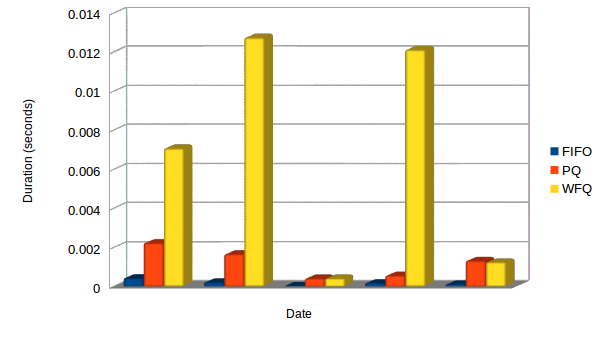
\includegraphics[width=0.5\textwidth]{duration}
\label{fig:duration}\caption{Average Durations per Date and Queue Type}
\end{figure}

It is evident from \ref{fig:duration} that in terms of how fast the packets are scheduled, \texttt{WFQ} takes the most time to finish in scheduling the packets. Duration \textit{d} is a function of the arrival time \textit{t\textsubscript{0}} and last switched time \textit{t\textsubscript{n}} seen as follows:

\[
	d(t_0, t_n) = t_n - t_0
\]

\subsubsection{Throughput}
\begin{figure}
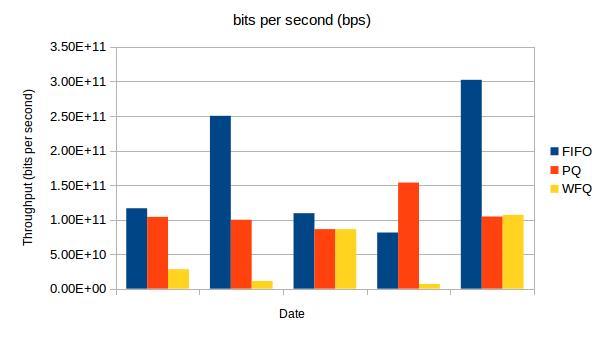
\includegraphics[width=0.5\textwidth]{throughput}
\label{fig:throughput}\caption{Average Throughputs per Date and Queue Type}
\end{figure}

Throughput \textit{tput} was computed as 
\[
	tput = \frac{count(p_s)}{d}
\]

where \textit{ts} is the total size (in bytes) that was successfully switched, and \textit{d} as the computed duration. Focusing on \ref{fig:throughput}, \texttt{FIFO} scheduling queue outputted the most throughput.

\subsubsection{Packet Loss}
\begin{figure}
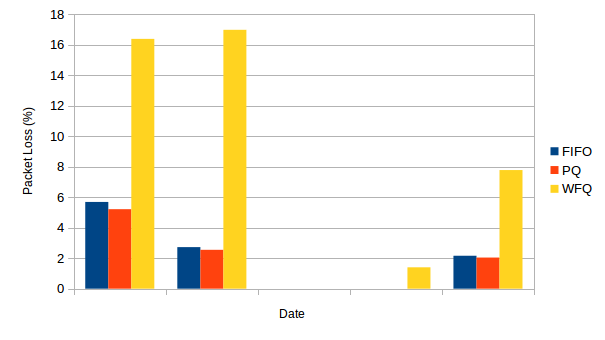
\includegraphics[width=0.5\textwidth]{packetloss}
\label{fig:packetloss}\caption{Average Packet Losses per Date and Queue Type}
\end{figure}

The last network performance parametric looked at is the packet loss \textit{l}, solved by

\[
	l = \frac{count(p_l)}{count(p_l + p_s)} \times 100
\]

where all dropped packets \textit{p\textsubscript{l}} are counted, divided by the total of dropped \textit{p\textsubscript{l}} and switched packets \textit{p\textsubscript{s}} multiplied by 100, to get the percentage. Similarly, the results show that \texttt{WFQ} has the worst performance when packet loss is considered. Notably, \texttt{PQ} shows lower packet loss compared to \texttt{FIFO}.

\subsubsection{Bandwidth Constraint}
In attempt to check if the same trend is observed when a bandwidth constraint is added, the following bandwidth constraints were tested using a 100MBps buffer: 600Mbps, 800Mbps, 1000Mbps, and 1200Mbps. These values were converted into their byte form and with help from the conversion value for seconds to ticks, they were translated into 1.125 Bytes per tick (Bpt), 1.5Bpt, 1.875Bpt, and 2.25Bpt respectively. The result is visualized in \ref{fig:bc}. The throughputs noted for all ran simulations are very close to the bandwidth, and a 100MB buffer provided 0\% packet loss, hence only the duration was left as  basis.

As seen, PQ and WFQ amounted to the same duration that showed improvement per increase of the bandwidth. Yet, it is apparent that FIFO's performance is a lot better based on this network performance metric. FIFO, in any of the bandwidth constraints, displayed minimal and fast speed of switching the packets, while maintaining a similar throughput to the slow-performing PQ and WFQ.

\begin{figure}
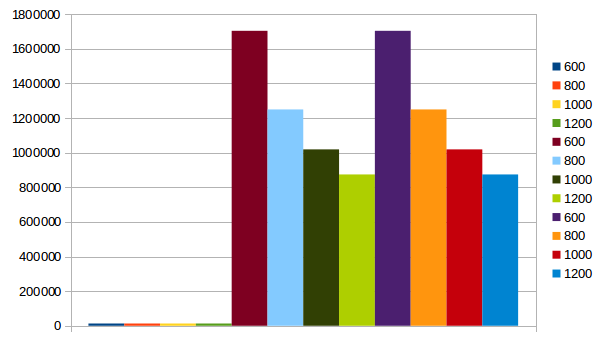
\includegraphics[width=0.5\textwidth]{duration_with_bc}
\label{fig:bc}\caption{Average Durations with Applied Bandwidth Constraint}
\end{figure}

\section{Conclusion and Recommendation}
After the experiment, the results show that the UPLB network works better using the \texttt{FIFO} scheduling algorithm. It was able to output the most number of packets over a period of time, as shown by \ref{fig:throughput}, and switched the packets fastly \ref{fig:duration} while maintaining the most integrity by minimizing lost packets\ref{fig:packetloss}.

While \texttt{PQ} and \texttt{WFQ} algorithms were intended to improve the network performance in terms of packet switching, this study proves that the traffic of UPLB is more suited to a \texttt{FIFO} scheduling algorithm.

For future studies, the researcher would recommend that a different traffic classification method is to be used, such as statistical methods or machine learning methods. Another advisable method is to inspect a different field of the payload or packet that will be used to classify traffic, instead of the protocol field. A final recommendation is the use of hybrid or variation of the PQ and WFQ scheduling algorithms to further improve the switching, thus effectively managing UPLB's internet bandwidth.

% BIBLIOGRAPHY
\bibliographystyle{./IEEE/IEEEtran}
\bibliography{./cs190-ieee}
% \nocite{*}

% BIOGRAPHY
\begin{biography}[{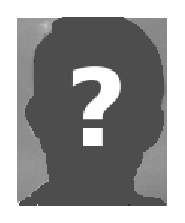
\includegraphics{./yourPicture.eps}}]{\ADVISEE}
She is a BS Computer Science undergraduate student. She not only writes code, but also songs, poems, and stories.
\end{biography}

\end{document}
